\documentclass[12pt,a4paper]{article}

\usepackage[english]{babel} %other options: frenchb,german,english
\usepackage[pdftex]{graphicx}
\usepackage[utf8]{inputenc}
\usepackage{hyperref}
\usepackage{listings}
\usepackage{geometry}
\usepackage{epstopdf}
\usepackage{amsmath}
\usepackage{hhline}
\usepackage[table]{xcolor}
\usepackage{makeidx}
\usepackage{unifrbr}
\usepackage[parfill]{parskip}
\usepackage[nottoc,notlof,notlot]{tocbibind}

\newcommand*{\captionsource}[2]{%
  \caption[{#1}]{%
    #1%
    \\\hspace{\linewidth}%
    \textbf{Source:} #2%
  }%
}

%\renewcommand{\baselinestretch}{1.5}
% Augmenter profondeur des sous-sections
%\setcounter{secnumdepth}{5}
%\setcounter{\tocdepth}{4}

\pagestyle{empty}
\renewenvironment{abstract}
 {\small
  \begin{center}
  \bfseries \abstractname\vspace{-.5em}\vspace{0pt}
  \end{center}
  \list{}{
    \setlength{\leftmargin}{.5cm}%
    \setlength{\rightmargin}{\leftmargin}%
  }%
  \item\relax}
 {\endlist}
\begin{document}

\sloppy
\renewcommand{\thepage}{}
\pagestyle{empty}

%----------------------------------------------------------------------------
\title{SocialMovies Mini-project  Web Engineering 2015}
\date{\today}
\author{Nadia \textsc{Aebsicher} \\ Simon \textsc{Brulhart} \\Jocelyn \textsc{Thode}\\}

\graphicspath{{figures/}}

\maketitle

%----------------------------------------------------------------------------
\pagenumbering{roman}
\pagestyle{plain}
\tableofcontents
%\listoffigures
%\listoftables
\newpage

%----------------------------------------------------------------------------
\pagenumbering{arabic}
\pagestyle{headings}


%############################################################################

\section{Introduction}

We used Ruby on Rails and RDF to create this project. The resulting web application lets you search movies, favorite and share them with your friends as well as getting personalized recommendations based on what you liked. You can also add movies to different lists such as 'Watch it later' or 'Watched'.

In the two next chapter, we will present our development environment as well as the different technologies used for the project. In chapter \ref{framework}, we will present the Ruby on Rails framework and explain how the MVC architecture works.

In chapter \ref{rdf}, we will present which RDF database we used and why RDF is useful.

In chapter \ref{app}, we will talk about our application, how it works and some interesting features.

Chapter \ref{install} will be about the installation and user guides. Finally we will conclude the report and reflect on what was achieved for this mini-project.

\section{Development Platform}\label{dev_plat}

The WEBrick web server coming with Ruby makes the application reachable at \url{http://localhost:3000}.

The development of the application was done with:
\begin{itemize}
\item \textbf{Operating Systems}: Mac OS X 10.11.1, Archlinux
\item \textbf{Web Browsers}: Safari 9.0.1, Chromium 47.0, Firefox 42.0
\end{itemize}



\section{Development Environment}\label{dev_plat}

We used the following environments to develop our application :

\begin{itemize}
\item \textbf{Ruby 2.2.3} is the programming language used by Rails
\item \textbf{Rails 4.2.4} is an MVC framework written in Ruby. It lets you develop web applications using the DRY (Don't Repeat Yourself) philosophy and the CRUD (Create Read Update Delete) system.

\item \textbf{SQLite 3.9} is a really simple RDMS that is ACID-compliant. We chose SQLite due to the fact it is contained in a single file and is really light.
\item \textbf{LinkedMDB} is the RDF database we chose to use to retrieve information about movies.
\item \textbf{OMDB} is a RESTful API to access data from the Internet Movie Databse.
\item \textbf{Redis} is a very fast in-memory key-value store with optional persistence.
\item \textbf{Git} via Github service for revision control.
\item \textbf{Atom} is a simple textditor with syntax highlighting.
\end{itemize}

% \section{Development Platform and Environment}\label{dev_plat_env}

% We used the following environments to develop our application :

% \begin{itemize}
% \item \textbf{Operating Systems}: Mac OS X 10.11.1, Archlinux
% \item \textbf{Web Browsers}: Safari 9.0.1, Chromium 47.0, Firefox 42.0
% \item \textbf{Ruby 2.2.3} is the programming language used by Rails
% \item \textbf{Rails 4.2.4} is an MVC framework written in Ruby. It lets you develop web applications using the DRY (Don't Repeat Yourself) philosophy and the CRUD (Create Read Update Delete) system.

% \item \textbf{SQLite 3.9} is a really simple RDMS that is ACID-compliant. We chose SQLite due to the fact it is contained in a single file and is really light.
% \item \textbf{HTML 5} 
% \item \textbf{CSS 3}
% \item \textbf{jQuery} is a fast, small, and feature-rich JavaScript library.
% \item \textbf{Bootstrap 3} is the CSS framework used to design the web pages. It lets us have a sleek design with minimal efforts.
% \item \textbf{LinkedMDB} is the RDF database we chose to use to retrieve information about movies.
% \item \textbf{OMDB} is a RESTful API to access data from the Internet Movie Databse.
% \item \textbf{Redis} is a very fast in-memory key-value store with optional persistence.
% \end{itemize}

% \begin{figure}[h]
% \begin{center}
% \fbox{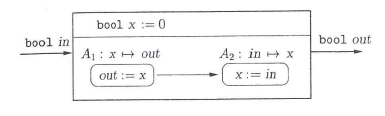
\includegraphics[scale=0.7]{splitdelay.png}}
% \end{center}
% \caption{\textbf{Delay component}}
% \label{splitdelay}
% \end{figure}

\section{Framework and MVC Pattern}\label{framework}
\subsection{Ruby on Rails}
As stated earlier Ruby on Rails is a framework following the MVC pattern using Ruby. It is really simple to use and does a lot of work on the back end to let the developer fully focus on their code without worrying about every details like security or how to link different objects together.

In short, it gives a really high-level interface to developers to create a web application.
\subsection{MVC}
The Model-View-Controller (MVC) separates the view from the applications's logic.

\subsubsection{Model}
The model does the application's business logic. It has to handle data (storing and retrieving). In Rails the Model is implemented through Active Record which is a class that wraps the database access in a Ruby object for ease of use.

Active Record also has great tools that let you handle the validations and the relationships between tables directly in the model. These validations and foreign keys are only present in the model layer this way and you will not have a foreign key present in the database.

In our project, the model layer was a bit more complicated to implement as we were using an external database namely the RDF database exposed by LinkedMDB. We had to retrieve information directly from LinkedMDB using the gem RDF.rb and sparql, and link the movie to our Active Record movie object so we could take advantage of different possibilities given by Active Record. This was especially useful for all the recommendation part.

\subsubsection{View}
The view should only serve to encapsulate the presentation logic. We should not do any application logic (Controller) or information retrieval through the database (Model). In our project, the view only displays the movie information given by the controller.

\subsubsection{Controller}
The controller is the link between the view and the model. It will retrieve information from the model, apply some transformations to it and pass it to the view.

\section{RDF}\label{rdf}
RDF stands for Resource Description Framework and is a W3C specification. It is a model used to link together web resources. The format to present such data is often N-Triples, meaning the information is separated in three pieces :
\begin{itemize}
\item The subject
\item The predicate
\item The object
\end{itemize}

RDF also links resources in a way that is easy for a computer to interpret as well as for a human. For example you can describe your \textit{person} resource with the class \texttt{Person} of the \texttt{foaf} ontology, and then a third-party service using the same ontology could understand that your resource represents a person, that its \texttt{lastName} property is the actual last name of the person, etc.

In our project we make use of such a RDF graph to search for movies using different criterias like the release year or the actors.

\section{SocialMovies Application}\label{app}

In this chapter we will look at different parts of our project that think are interesting.

\subsection{Database and Models}
The database in our project is mixed. We use models and SQLite to store the different lists, and to store the RDF movie ids as well as to store users. To get all the actual movie information we query the LinkedMDB using SPARQL queries. We also get the movie poster and plot from IMDB using the OMDB API (see Figure \ref{movie_info}).

\begin{figure}[h]
\begin{center}
\fbox{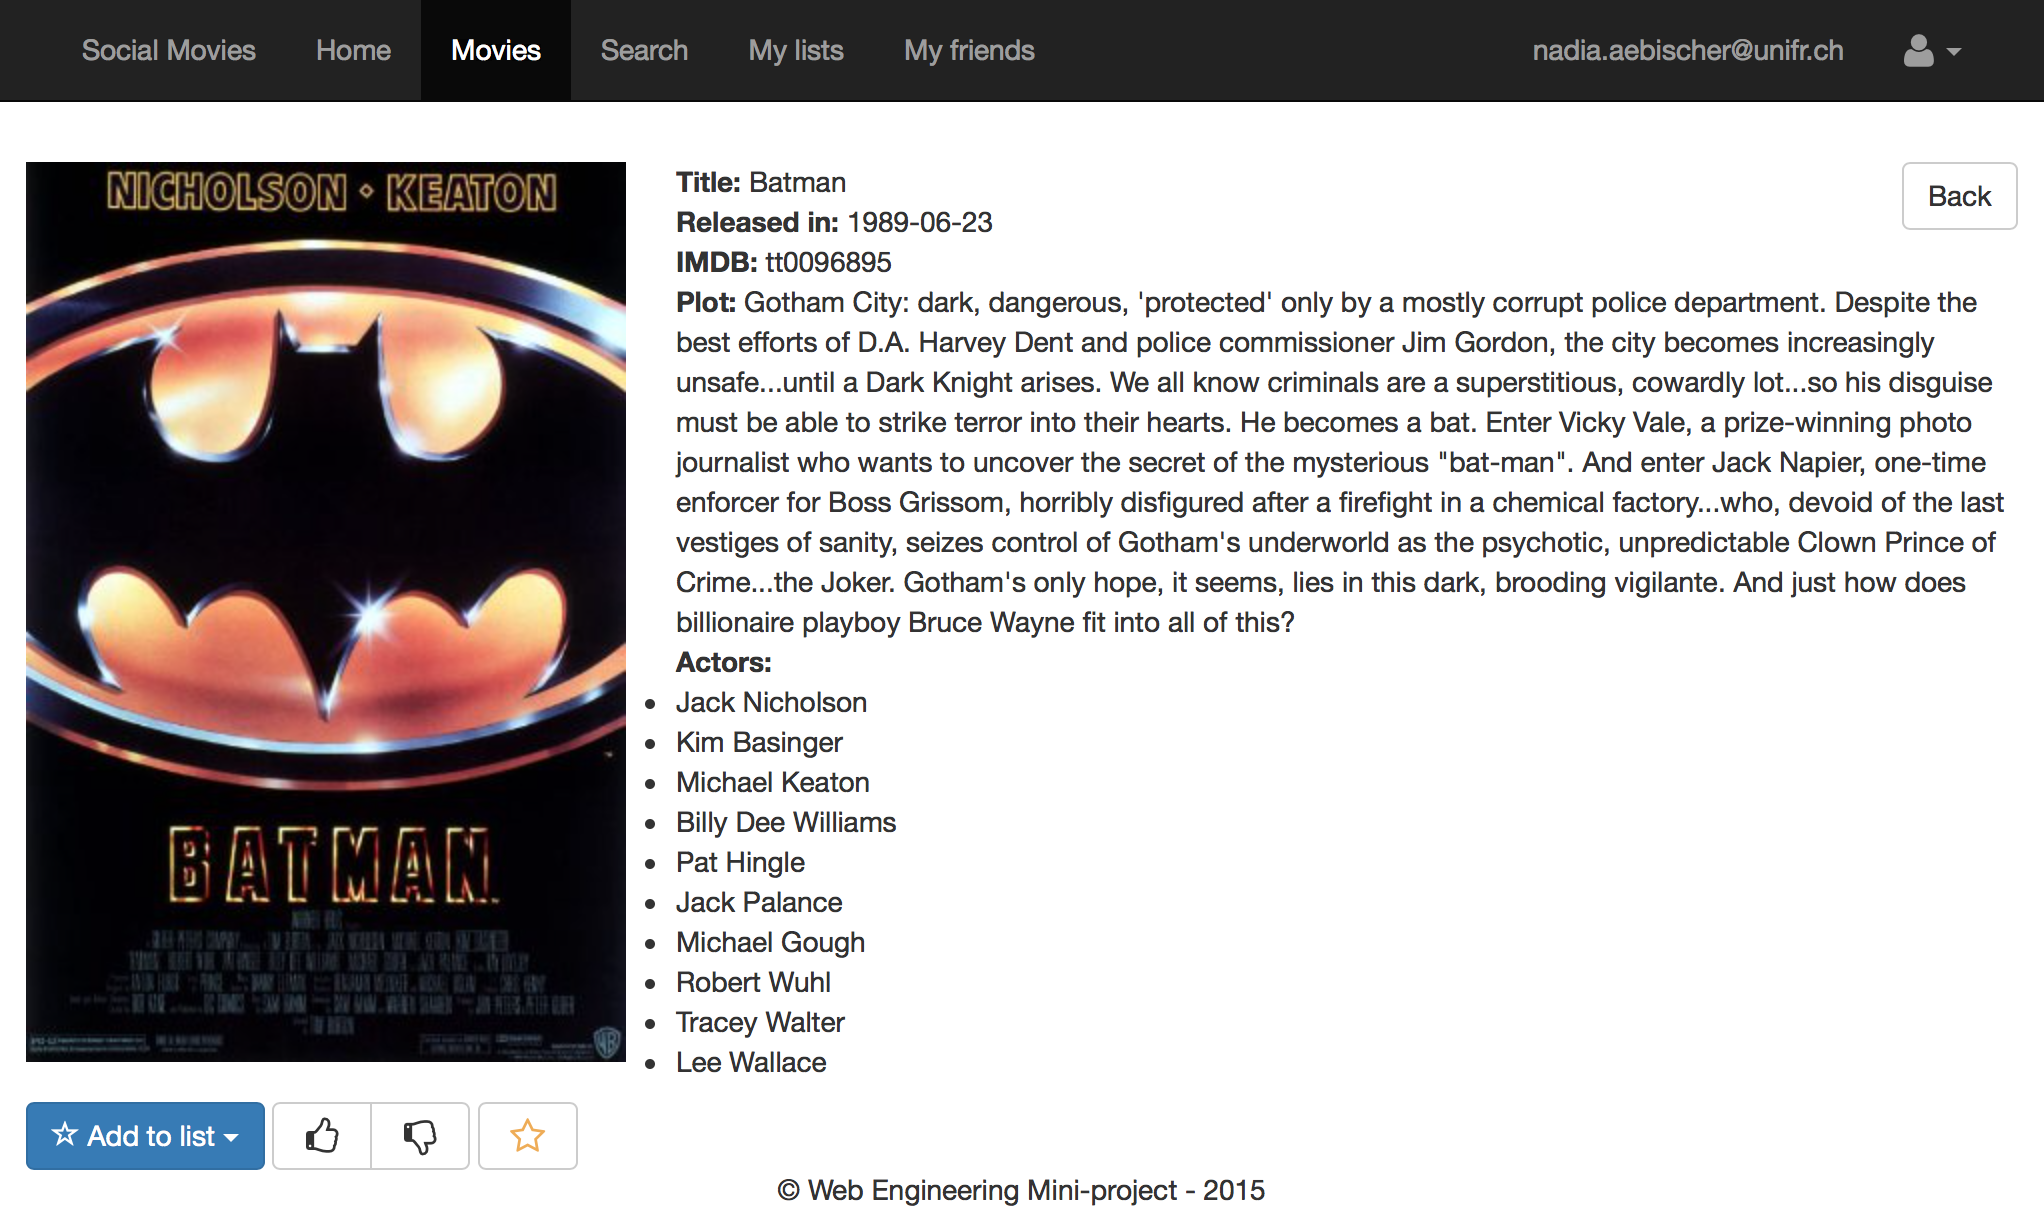
\includegraphics[scale=0.4]{movie_info.png}}
\end{center}
\caption{\textbf{Movie information}}
\label{movie_info}
\end{figure}

We have to store the movie IDs in a model, because we need to somehow retain which movie a user liked so that we can give him recommendations.

Gathering data from LinkedMDB and OMDB for each request can be costly whereas most of the retrieved never changes, so we cache every request using Redis.

\subsection{User Authentication}
The user authentication is a critical part of a web application. It is essential to secure this part to the best of your capabilities.

To ensure that, we used a gem called \textit{Devise} that manages authentication for us. This gem takes care of registration and signing in. It also stores the passwords in the database using strong encryption.

\subsection{Movies}
\subsection{Recommendations}
We wanted to be able to provide movies recommendations to a user based on what they liked (see Figure \ref{recommendation}). This can get pretty complicated as you have to create graphs and use data-mining techniques to emerge a relation graph between users.

\begin{figure}[h]
\begin{center}
\fbox{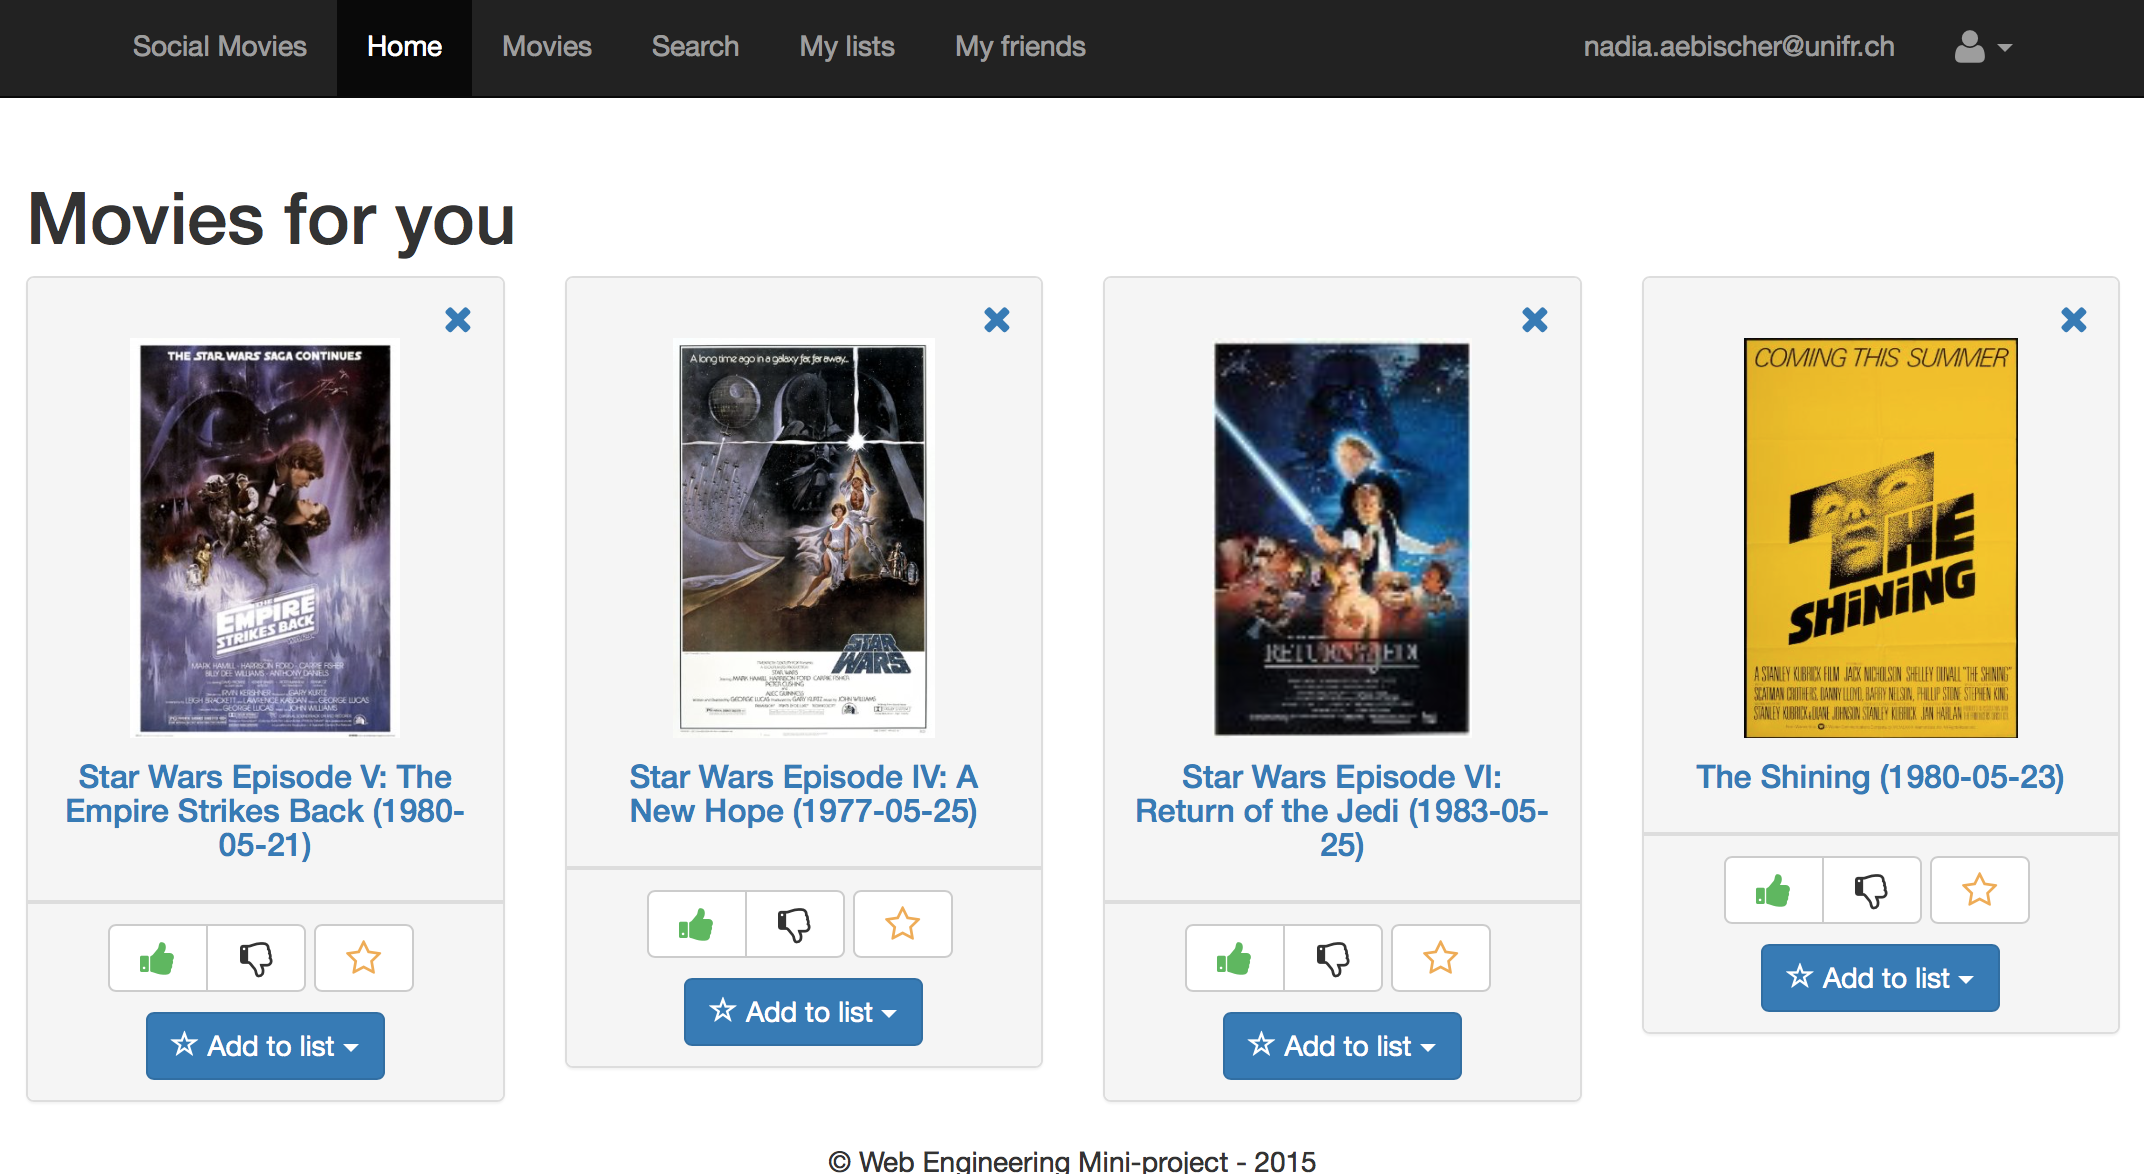
\includegraphics[scale=0.4]{recommendation.png}}
\end{center}
\caption{\textbf{Movie recommendations}}
\label{recommendation}
\end{figure}

\subsubsection{Recommendable}
Fortunately a gem called \textit{Recommendable} exists. It takes care of all the relationships and just gives you which items a user might like based on what they have liked previously.

In SocialMovies, you can either like, dislike or hide a movie. Based on these three actions, recommendable will generate a list of the recommended movies for you to see.

The gem uses Redis and Sidekiq in the backend. Sidekiq is a gem that lets you easily schedule background jobs.

Redis is used to store the relationships between users for the recommendation part. Sidekiq is used to update the recommendations for each users. Obviously this task has to be done in the background, otherwise the application would become really slow.

\subsubsection{Lists}
In our project we have implemented lists (see Figure \ref{mylists}) for a user to save movies they want to watch later, movies they have as favorites etc.

\begin{figure}[h]
\begin{center}
\fbox{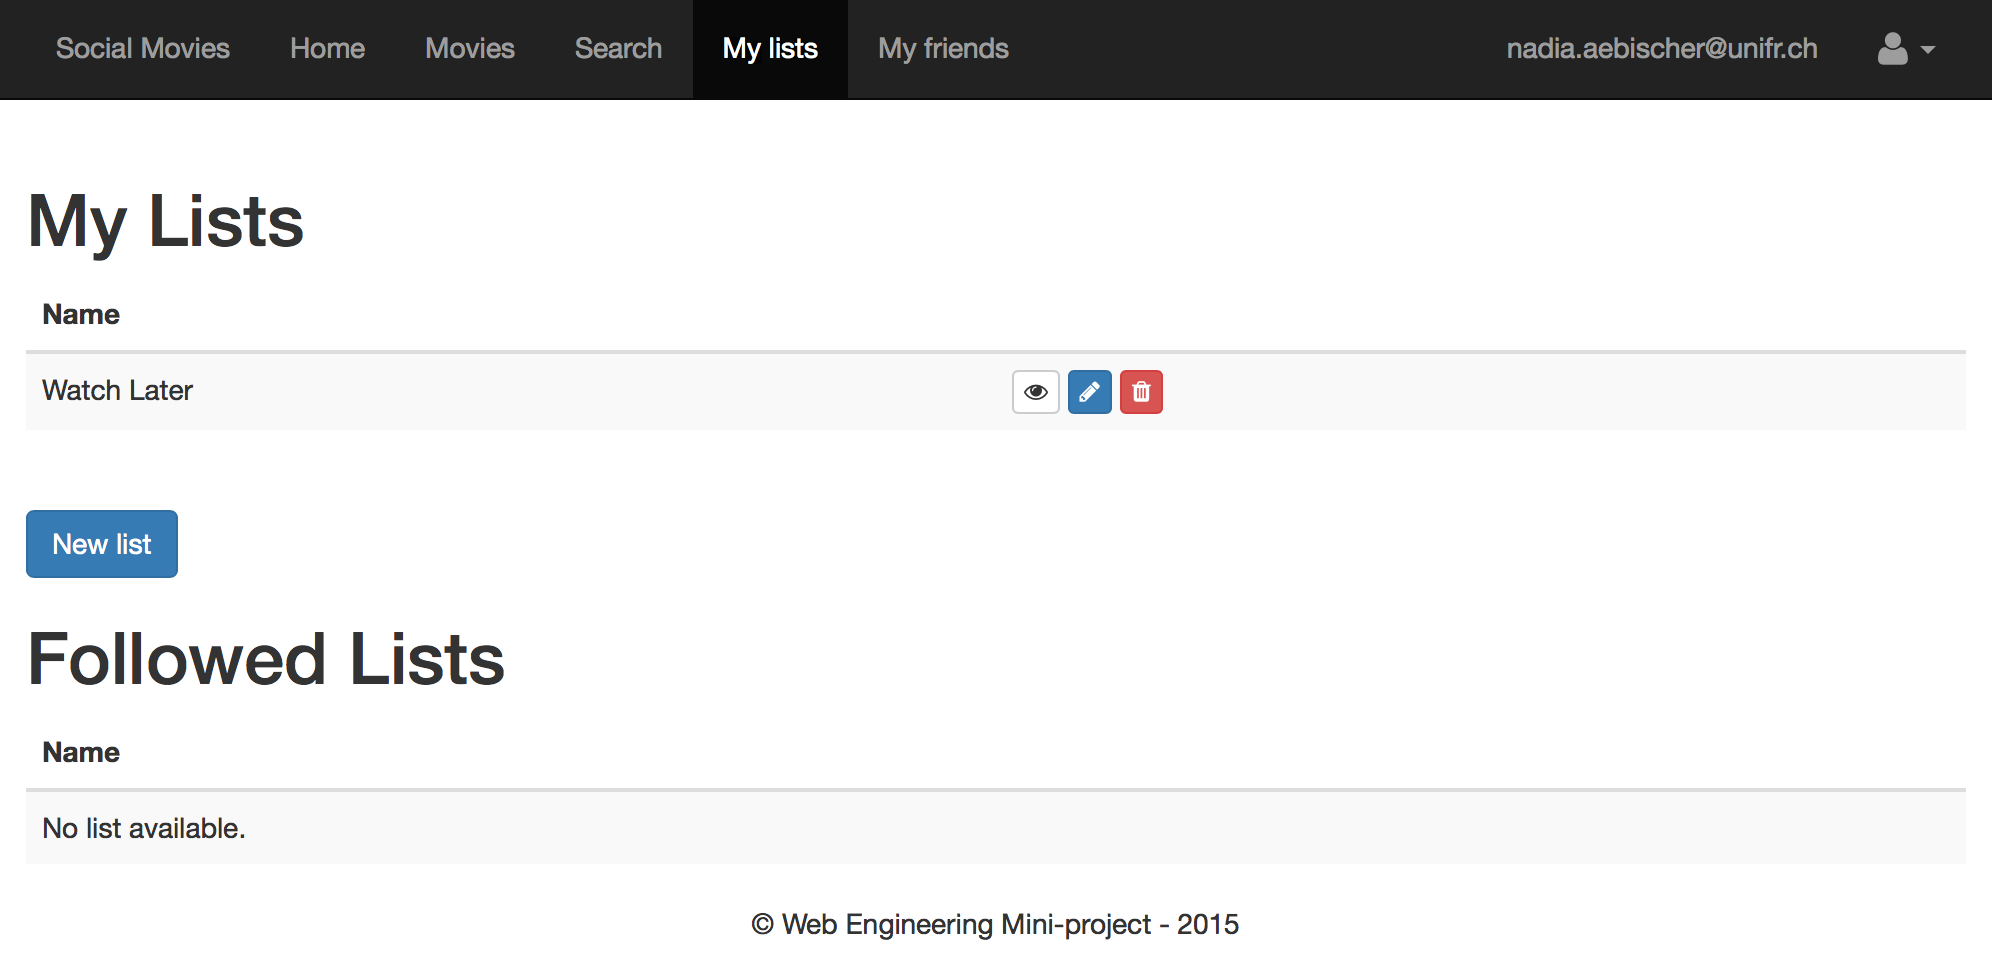
\includegraphics[scale=0.4]{mylists.png}}
\end{center}
\caption{\textbf{User's lists}}
\label{mylists}
\end{figure}

Users can add movies to the list they want and remove them at any time. The favorite list is also used to recommend movies. Users can also create their own lists, follow the lists of other users, see the lists of their friends, etc (see Figure \ref{myfriends_follow}).

\begin{figure}[h]
\begin{center}
\fbox{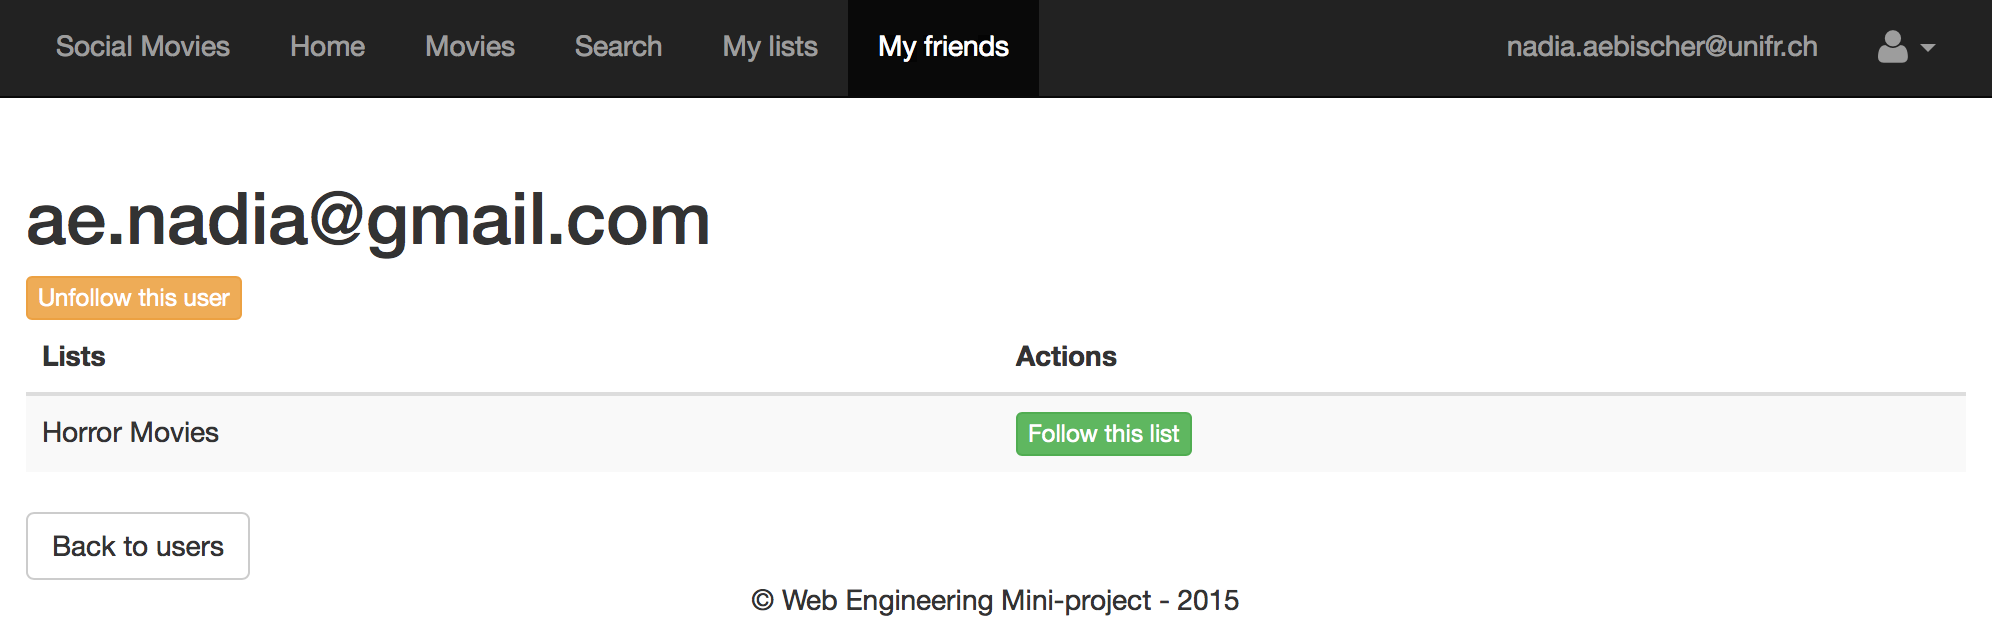
\includegraphics[scale=0.4]{myfriends_follow.png}}
\end{center}
\caption{\textbf{Follow lists and friends}}
\label{myfriends_follow}
\end{figure}

\section{Guides}\label{install}

\subsection{Installation Guide}
In order to run the web application you need to :
\begin{enumerate}
\item Install SQLite 3
\item Install Ruby $>=$ 2.2
\item Install Rails 4.2.4
\item Install Redis
\item Install the gem Bundler
\item Copy the SocialMovies directory from the usb stick or clone it from \href{https://github.com/jocelynthode/SocialMovies}{https://github.com/jocelynthode/SocialMovies}
\item Go to the SocialMovies directory and type : \begin{lstlisting} 
bundle install 
\end{lstlisting}
\item Create the database by running in your terminal :
\begin{lstlisting} 
rake db:create && rake db:migrate
\end{lstlisting}
\item start redis with :
\begin{lstlisting} 
redis-server &
\end{lstlisting}
\item start sidekiq with :
\begin{lstlisting} 
bundle exec sidekiq -q recommendable &
\end{lstlisting}
\item start the application :
\begin{lstlisting} 
bin/rails server
\end{lstlisting}
\end{enumerate}
\subsection{User Guide}
To start using the app, you must register using the \textit{Sign Up} button. After that you can start browsing and searching for different movies. The more movies you like/dislike and add to your lists, the more precise the recommendations will get.

%TODO

\section{Conclusion}
To conclude this report, we have implemented a web application that lets a user search for movies, get recommendations and use lists to save movies to watch later. We used Ruby on Rails + Bootstrap as the framework and RDF databases to retrieve movie information.

We were already familiar with Ruby on Rails before this project, but had never used RDF. RDF has some really good ideas and is really generic which makes it easy to use in multiple completely different applications. 

We still had problems with it, mainly due to the fact that most open link RDF databases are either out of date (LinkedMDB has not been updated for more than three years) or have missing information. To palliate to these problems we had to rely on third party APIs that are not using RDF, such as OMDB.

Using SPARQL for the first time was also challenging, because it was not exactly like SQL which we are used to.

In the end we enjoyed working with Ruby on Rails and RDF and we wish there would be more services providing a SPARQL end-point and using RDF to structure their data.




%############################################################################
\newpage
\begin{thebibliography}{20}

\bibitem{rdfwiki}
\href{https://en.wikipedia.org/wiki/Resource\_Description\_Framework}{https://en.wikipedia.org/wiki/Resource\_Description\_Framework}

\bibitem{railswiki}
\href{https://en.wikipedia.org/wiki/Ruby\_on\_Rails}{https://en.wikipedia.org/wiki/Ruby\_on\_Rails}

\bibitem{railswiki}
\href{https://en.wikipedia.org/wiki/Model\%E2\%80\%93view\%E2\%80\%93controller}{https://en.wikipedia.org/wiki/Model–view–controller}
\end{thebibliography}

\end{document}
